\chapter{Estimadores}
Recordemos que, dada una familia de modelos estadísticos y datos que asumimos vienen de un miembro de dicha familia, nuestro objetivo es obtener (estimar) el modelo particular que generó los datos, es decir, cuáles son los parámetros del modelo. En este capítulo se introducirá la noción de estimador, es decir, una función que busca estimar el parámetro mencionado anteriormente en base a los datos disponibles.

\begin{definition}
    Sea $g:\Omega\rightarrow \mathbb{R}^n$  tal que $g(\theta) = (g_1(\theta),...,g_n(\theta))$ a valores en $\mathbb{R}$. Nos interesa estimar $g(\theta)$. Para estimar $g(\theta)$ usamos un \textbf{estimador} que es una función $\hat{g}:\mathfrak{X}\rightarrow g(\Omega)$ medible. Diremos que $\hat{g}(\theta)$ es la estimación de $g(\theta)$.
    
\end{definition}

\begin{remark}
    Los estimadores son casos particulares de los estadísticos, pues son funciones de los datos que tienen por conjunto de llegada la imagen de $\Omega$ a través de $g(\cdot)$.
\end{remark}

\begin{remark}
    Los estimadores pueden ser usados para estimar el parámetro propiamente tal, en cuyo caso $g(\theta)=\theta$, o bien otras cantidades del modelo que son expresables a través de los parámetros. Por ejemplo, en el caso de un modelo Gaussiano, si bien el parámetro puede ser expresado como $\theta = [\mu,\sigma^2]$, podemos estar interesados en estimar el intervalo de confianza del 95\%, el cual está dado (aproximadamente) por 
    \begin{equation}
        g(\theta) = [\mu - 2\sigma,\mu + 2\sigma].
    \end{equation}
\end{remark}

\begin{example}[Estimador de la media Gaussiana]
	\label{ex:estimador_media}
	Consideremos $X = (X_1,\ldots,X_n)\sim\cN(\mu,\sigma^2)$. Un estimador de $g(\theta) = g(\mu,\sigma) = \mu$ es el estadístico 
	\begin{equation}
	\nonumber
		\gh(X) = \frac{1}{n}\sum_{i=1}^nX_i.
	\end{equation} 
\end{example}



\section{Estimadores insesgados} 
Recordemos que nuestros estimadores, como función de la variable aleatoria $X$, son a su vez variables aleatorias. Consecuentemente, su estudio debe considerar sus propiedades aleatorias también. El primer paso para esto es la siguiente definición que dice relación con el valor esperado del estimador y el valor de la función $g(\theta)$ que éste estima. 

\begin{definition}[Estimador insesgado]
	\label{def:estimador_insesgado}
	Sea $\ghX$ un estimador de $g(\theta)$. Este estimador es insesgado si 
	\begin{equation}
	\nonumber
		\E{\ghX} = g(\theta),
	\end{equation}
	donde el \emph{sesgo} de $\gh$ se define como 
	\begin{equation}
	\nonumber
		b_\gh(\theta) = \E{\ghX} - g(\theta).
	\end{equation}
	Se dice también que un estimador es \textbf{asintoticamente insesgado} si es que:
	\[\lim_n\E{\gh (X_1,...,X_n)} = g(\theta),\]
	es decir, si el estimador solo se convierte en insesgado al usar \emph{infinitos datos}.
\end{definition}

Los estimadores insesgados juegan un rol relevante en el estudio y aplicación de la estadística, pues nos dicen que el estimador recupera efectivamente el parámetro \emph{en promedio}. Sin embargo, uno no siempre debe poner exclusiva atención a ellos, pues el hecho que funcione en promedio no garantiza nada en cuanto a su dispersión (varianza) o cuántas muestras necesitamos para que el estimador sea confiable. 

Los siguientes ejemplos ilustran el rol del estimador insesgado en dos familias paramétricas distintas. 

\begin{example}[Estimador insesgado de la media Gaussiana]
	\label{ex:estimador_in_media}
	El estimador de $g(\theta) =  \mu$ descrito en el Ejemplo \ref{ex:estimador_media} es insesgado, en efecto: 
	\begin{equation}
	\nonumber
		\E{\ghX} = \E{\frac{1}{n}\sum_{i=1}^nX_i}	= \frac{1}{n}\sum_{i=1}^n\E{X_i}		= \frac{1}{n}\sum_{i=1}^n\mu = \mu.
	\end{equation}
\end{example}




Veamos ahora un ejemplo de un estimador \textbf{sesgado} de la varianza y cómo se puede construir un estimador insesgado en base a éste. 

\begin{example}
Consideremos una familia paramétrica $\familiaparametrica$ y denotemos por $\mu$ y $\sigma^2$ su media y su varianza respectivamente. Usando las observaciones $x_1,x_2,\ldots,x_n$, calculemos la varianza del estimador de la media, dado por $\xb = \frac{1}{n}\sum_{i=1}^n x_i$ mediante
\begin{equation}
	\label{eq:varianza_media_muestral}
 	\Vt{\xb} = \Vt{\frac{1}{n}	\sum_{i=1}^n x_i}  \underbrace{=}_{\text{i.i.d.}}  \frac{1}{n^2}	\sum_{i=1}^n\Vt{ x_i} =\frac{\sigma^2}{n}
 \end{equation} 
 es decir, el estimador de la media usando $n$ muestras, tiene una varianza $\sigma^2/n$.

 Consideremos ahora el siguiente estimador para la varianza: 
\begin{equation}
	\label{eq:est_varianza_sesgado}
	S_2 = \frac{1}{n}\sum_{i=1}^n (x_i-\xb)^2
\end{equation}
y notemos que la esperanza de dicho estimador es
\begin{align}
	\label{eq:sesgo_varianza}
	\Et{S_2 } &= \Et{\frac{1}{n}\sum_{i=1}^n (x_i-\mu+\mu-\xb)^2}\nonumber\\
				&= \Et{ \frac{1}{n}\sum_{i=1}^n(x_i-\mu)^2 + 2\frac{1}{n}\sum_{i=1}^n(x_i-\mu)(\mu-\xb) + \frac{1}{n}\sum_{i=1}^n(\mu-\xb)^2}\nonumber\\
				&= \Et{ \frac{1}{n}\sum_{i=1}^n(x_i-\mu)^2 - 2(\mu-\xb)^2 + (\mu-\xb)^2}\nonumber\\
				&= \Et{ \frac{1}{n}\sum_{i=1}^n(x_i-\mu)^2 - (\mu-\xb)^2}\nonumber\\
				&= \Vt{x_i} - \Vt{\xb}\quad\text{ver ecuación \eqref{eq:varianza_media_muestral}}\nonumber\\
				&= 	\sigma^2 + \sigma^2/n = \left(\frac{n+1}{n}\right)\sigma^2
\end{align}
Esto quiere decir que el sesgo del estimador en la ecuación \eqref{eq:est_varianza_sesgado} es asintóticamente insesgado, es decir, que su sesgo tiende a cero cuando el número de muestas $n$ tiende a infinito. Sin embargo, notemos que podemos corregir el estimador de la varianza multiplicando el estimador original, $S_2$ en la ecuación \eqref{eq:est_varianza_sesgado} por $n/(n+1)$, con lo que el estimador corregido denotado por 
\begin{equation}
	\label{eq:est_varianza_insesgado}
	S'_2 = \frac{n}{n+1}S_2 =  \frac{1}{n+1}\sum_{i=1}^n (x_i-\xb)^2
\end{equation}
cumple con
\begin{equation}
	\Et{S'_2 } =  \left(\frac{n}{n+1}\right)\Et{S_2} \underbrace{=}_{\text{ec.}\eqref{eq:sesgo_varianza}} \left(\frac{n}{n+1}\right) \left(\frac{n+1}{n}\right)\sigma^2 = \sigma^2
\end{equation}
es decir, el estimador $S'_2$ en la ecuación \eqref{eq:est_varianza_insesgado} es insesgado.
\end{example}

\section{Completitud}

Otra propiedad de los estimadores que permite estudiar su capacidad de estimar es la de \textit{completitud}. A continuación definimos esta propiedad para el caso general de un estadístico, no necesariamente un estimador.

\begin{definition}[Estadístico completo]
	Un estadístico $T(X)$ es completo si para toda función $f$, se tiene que 
	\begin{equation}
		\Et{f(T)|\theta} = 0, \forall \theta\in\Theta \Rightarrow \Probt{f(T)=0} = 1, \forall \theta\in\Theta.
	\end{equation}
	
\end{definition}

Intuitivamente entonces, podemos entender la noción de completitud como lo siguiente: un estadístico es completo si la única forma de construir un estimador insesgado de cero a partir de él es aplicándole la función idénticamente nula.  Veamos un ejemplo de la distribución Bernoulli, donde el estadístico $T(x) = \sum x_i$ es efectivamente completo. 

\begin{example}
	\label{eq:est_completo_bernoulli}
	Sea $x=(x_1,\ldots,x_n)$ observaciones de $X\sim\ber{\theta}$, recordemos que $T(x) = \sum x_i\sim\bin{n,\theta}$, por lo que la esperanza de $f(T)$ está dada por
	\begin{equation}
		\Et{f(T)} = \sum_{t=0}^n f(t)\binom{n}{t}\theta^t(1-\theta)^{n-t}= (1-\theta)^n\sum_{t=0}^n f(t)\binom{n}{t}\left(\frac{\theta}{1-\theta}\right)^t,
	\end{equation}
	es decir un polinomio de grado $n$ en $r=\theta/(1-\theta)\in\R_+$. Entonces, $\Et{f(T)} = 0,\forall\theta$, implica que necesariamente los pesos de este polinomio son todos idénticamente nulos, es decir, $f(t)=0,\forall t$, lo que a su vez implica $\Probt{f(T)=0} = 1$. Consecuentemente, $T(x) = \sum x_i\sim\bin{n,\theta}$ es un estadístico completo.
\end{example}

El concepto de completitud dice relación con la construcción de estimadores usando estadísticos, lo cual puede ser ilustrado mediante el siguiente ejemplo

\begin{example}
	Consideremos dos estimadores, $\phi_1, \phi_2$ insesgados de $\theta$ distintos, es decir, 
	\begin{equation}
	\E{\phi_1} = \E{\phi_2} = \theta, \ \Prob{\phi_1\neq \phi_2} > 0.
	\end{equation}
	Definamos ahora $\phi = \phi_1 - \phi_2$, donde verificamos que $\E{\phi} = 0, \forall \theta$, es decir, $\phi$ es un estimador insesgado de cero. Como nuestra hipótesis en la ecuación anterior dice que $\Prob{\phi_1 - \phi_2=0}>0$, de acuerdo a la definición  de estadístico completo, $\phi$ no es completo. 
\end{example}


\begin{example}[Estimador de la taza de la distribución exponencial]
	\label{ex:estimador_exponancial}
	Consideremos $X\sim Exp(\theta)$, donde $Exp(x|\theta) = \theta\exp(-\theta x),\theta>0$. Veamos en primer lugar que el estadístico trivial $T(X) = X$ es completo. En efecto, para una función cualquiera $f(\cdot)$, como $\theta>0$ tenemos
	\begin{equation}
	    \Et{f(X)} = \int_0^\infty f(x)\theta\exp(-\theta x)\d x = 0 \Rightarrow  \int_0^\infty f(x)\exp(-\theta x)\d x = 0
	\end{equation}
	con lo cual si el lado derecho de la expresión anterior se cumple  $\forall \theta$, entonces necesariamente $f(x)=0$ (¿por qué?).
	
	En segundo lugar, asumamos que existe un estimador insesgado $\ghX$ de $g(\theta) = \theta$. Es decir, 
	\begin{equation}
	\nonumber
		\Et{\ghX} = \int_0^\infty \ghx\theta\exp(-\theta x)\d x = \theta, \forall \theta,
	\end{equation}
	lo cual es equivalente a $\int_0^\infty \ghx\exp(-\theta x)\d x = 1, \forall \theta$, y también a (al derivar ambos lados de esta expresión c.r.a. $\theta$) 
	\begin{equation}
	    \int_0^\infty x\ghx\exp(-\theta x)\d x = 0, \forall \theta.
	\end{equation}

	Esta última expresión es equivalente a que $\E{X\ghX} = 0$, con lo que podemos utilizar el hecho de que $X$ es un estadístico completo para decir que la función $X\ghX=0$ c.s. $\forall \theta$, y consecuentemente $\ghX=0$ c.s. $\forall \theta$. 
	
	Hemos mostrado que el supuesto de la existencia de un estimador (denotado $\ghX$) insesgado para el parámetro del modelo exponencial $\theta>0$, resulta en la contradicción $\ghX=0$ c.s. Consecuentemente, no es posible construir estimadores insesgados para $\theta$ en la distribución exponencial.
\end{example}




\section{Funciones de pérdida}

Una función de pérdida, también llamada función de costo, es una función a valores reales de dos argumentos que, intuitivamente, determina el costo de estimar uno de los argumentos mediante el otro. Como nuestro objetivo es estimar parámetros definimos entonces una función de costo de la siguiente forma. \textbf{Desde ahora consideraremos estimadores de $g(\theta) = \theta$ y todas las esperanzas serán con respecto a $\theta$ por simplicidad de notación.}

\begin{definition}[Función de costo]
Sea $\theta\in\Omega$ un parámetro y $a\in\Omega$ un estimador, entonces el costo de estimar $\theta$ mediante $a$ está dado por la función de costo definida mediante:
\begin{align}
    L: (\Omega \times \Omega) &\rightarrow \R\\
    (\theta \times a) &\mapsto L(\theta,a).
\end{align}

\end{definition}

\begin{example}[Función de costo cuadrática]
	\label{ex:costo_cuadrático}
Una función de costo ampliamente usada para comparar estimadores es el \textbf{error cuadrático}, el cual
está dado por  
$$
L_2(\theta,a) = ||\theta-a||^{2}.
$$
\end{example}
Pregunta: ¿por qué usamos el exponente igual a 2 y no otro?

\begin{example}[Función de costo $0-1$]
	\label{ex:costo_0-1}
Cuando estimamos parámetros que no tiene relación de orden, podemos usar la función de costo $0-1$ dada por
$$
L_{01}(\theta,a) = \mathbb{1}_{\theta\neq a}.
$$
\end{example}

\begin{example}[Divergencia de Kullback-Liebler]
	\label{ex:costo_KL}
Cuando los parámetros a estimar son distribuciones de probabilidad, podemos usar la siguiente función de costo
$$
L_{\text{KL}}(\theta,a) = \sum_{i=1}^D\theta_i \log\left(\frac{\theta_i}{a_i}\right).
$$
\end{example}

	
Como el estimador (que es el argumento de la función de pérdida) es una VA, también lo es la función de pérdida.  Consecuentemente, podemos calcular la esperanza de la función de pérdida, lo cual conocemos como \textit{riesgo}. 

En particular, el riesgo asociado a la pérdida cuadrática en el Ejemplo \ref{ex:costo_0-1} para un estimador $\phi$ del parámetro $\theta$, está dado por: 
\begin{alignat}{3}
 	R(\theta, \phi)  &= \E{(\theta - \phi)^2}\nonumber\\
 						& = \E{\left(\theta - \bar{\phi}+ \bar{\phi} -\phi\right)^2}; \quad \text{denotando }\bar{\phi} = \E{ \phi}\nonumber\\
 						& = \E{(\theta - \bar{\phi})^2+2(\theta - \bar{\phi})\cancel{(\bar{\phi} -\phi)} +  (\bar{\phi} -\phi)^2}\nonumber\\
 						& = \underbrace{(\theta - \bar{\phi})^2}_{=b_{\phi}^2\ (\text{sesgo}^2)} +  \underbrace{\E{(\bar{\phi} -\phi)^2}}_{=V_{\phi}\ \text{(varianza)}}.\label{eq:riesgo_cuad}
 \end{alignat} 
 Donde podemos ver unas de las razones de la consideración del costo cuadrático: su riesgo se divide intuitivamente en dos términos que expresan la exactitud (cuán sesgado es) y la precisión (cuán disperso es) del estimador.

\section{Teorema de Rao-Blackwell}
\textbf{Comentario:} Para una notación más clara, nos referimos  a los estimadores estimadores $\phi=\gh$ de $\theta$ en general para evitar la expresión más engorrosa estimador $\gh(X)$ de $g(\theta)$.

Siguiendo el racional de la sección anterior, evaluaremos la bondad de distintos estimadores (sesgados o insesgados) mediante una función de \textit{pérdida} o \textit{costo} que compara el valor reportado por el estimador y el valor real del parámetro. Esto permite usar la función de pérdida como una métrica para comparar (la bondad de) dos o más estimadores.\\

El siguiente teorema establece que la información reportada por un estadístico suficiente (Definición \ref{def:estadístico_suficiente}), puede solo mejorar un estimador. 

\begin{theorem}[Teorema de Rao-Blackwell]
	\label{teo:rao-blackwell}
	Sea $\phi = \phi(X)$ un estimador de $\theta$ tal que $\Et{\phi}<\infty, \forall \theta$. Asumamos que existe $T=T(X)$ estadístico suficiente para $\theta$ y sea $\phi^\star = \Et{\phi|T}$. Entonces, 
	\begin{equation}
		\Et{(\phi^\star-\theta)^2} \leq \Et{(\phi-\theta)^2}, \forall\theta,
	\end{equation}
	donde la desigualdad es estricta salvo en el caso donde $\phi$ es función de $T$.
\end{theorem}

En otras palabras, el Teo. de Rao-Blackwell establece que un estimador puede ser \textit{mejorado} si es reemplazado por su esperanza condicional dado un estadístico suficiente. El proceso de mejorar un estimador poco eficiente de esta forma es conocido como \textit{Rao-Blackwellización} y veremos un ejemplo a continuación.


\begin{example}
Consideremos $X = (X_1,\ldots,X_n)\sim \poi{\theta}$ y estimemos el parámetro $\theta$. Para esto, consideremos el estimador básico $\phi = X_1$ y \textit{Rao-Blackwellicémoslo} usando el estimador suficiente $T=\sum_{i=1}^nX_i$, es decir, 
\begin{equation}
	\phi^* = \Et{X_1\middle|\sum_i X_i=t}.
\end{equation}
Para calcular esta esperanza condicional, observemos primero que  
\begin{equation}
	\sum_{j=1}^n\Et{X_j\middle|\sum_{i=1}^n X_i=t} = \Et{\sum_{j=1}^nX_j\middle|\sum_{i=1}^n X_i=t} = t,
\end{equation}
y que como $X_1,\ldots,X_n$ son iid, entonces todos los términos dentro de la suma del lado izquierdo de la ecuación anterior son iguales. Consecuentemente, recuperamos el estimador
\begin{equation}
 	\phi^* = \frac{t}{n} = \frac{1}{n}\sum_{i=1}^nX_i.
 \end{equation} 
\end{example}

Antes de demostrar el Teorema \ref{teo:rao-blackwell} consideremos dos variable aleatorias $X\in\cX$, $Y\in\cY$, y recordemos dos propiedades básicas. En primer lugar la ley de esperanzas totales, la cual establece que 
\begin{alignat}{3}
	\mathbb{E}_Y{\mathbb{E}_{X|Y}{(X|Y)}} &= \int_\cY\int_\cX x \d P(x|y) \d P(y) \quad\quad&&\text{def. esperanza}\nonumber\\
				&=  \int_\cX x \int_\cY \d P(x|y) \d P(y) &&\text{linealidad}\nonumber\\
				&=  \int_\cX x \int_\cY \d P(x,y) &&\text{def. esperanza condicional}\nonumber\\
				&=  \int_\cX x \d P(x) = \mathbb{E}_X(X). &&\text{def. esperanza} \label{eq:total_expectation}
\end{alignat}
En segundo lugar, recordemos (?) la desigualdad de Jensen, la cual para el caso particular del costo cuadrático, puede verificarse mediante
\begin{equation}
	0 \leq \V{X} =  \E{X^2}-\E{X}^2 \Rightarrow \E{X^2} \geq \E{X}^2. \label{eq:jensen_var}
\end{equation}
La desigualdad de Jensen es geométricamente intuitiva, como se observa en la Figura \ref{fig:intuicion_jensen}. Al calcular la imagen de $\mathbb{E}(x)$ bajo una función convexa, podemos encontrar una recta tangente a ese punto $L(X)=aX+b$. Tendremos que $\mathbb{E}(\varphi(X')) \geq \mathbb{E}(L(X'))=\mathbb{E}[aX'+b]=a\mathbb{E}[X`]+b=L(\mathbb{E}(X'))$ para otro punto $X'$. Tomando $X'=X$, $\mathbb{E}(\varphi(X)) \geq \varphi(\mathbb{E}(X))$.
\begin{figure}[ht]
    \centering
    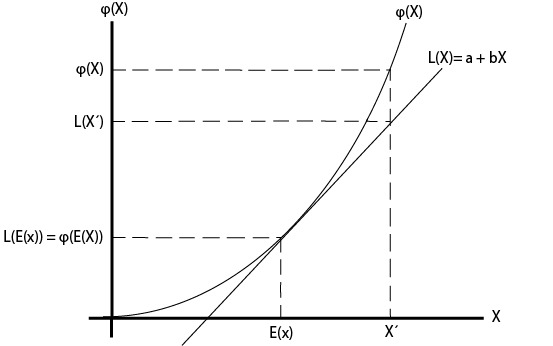
\includegraphics[scale=0.5]{img/Intuicion_Jensen.jpeg}
    \caption{Intuición geométrica de la desigualdad de Jensen }
    \label{fig:intuicion_jensen}
\end{figure}

Volviendo a lo anterior, utilizando las expresiones en \eqref{eq:total_expectation} y \eqref{eq:jensen_var}, podemos demostrar el teorema anterior.

 \begin{proof}[Demostración de Teorema \ref{teo:rao-blackwell}]
 	La varianza del estimador $\phi^\star$ está dada por 
 	\begin{alignat*}{2}
 		\Et{(\phi^\star-\theta)^2} &= \Et{(\Et{\phi|T}-\theta)^2} \quad\quad\quad &&\text{def.}\\
 								&= \Et{(\Et{\phi-\theta|T})^2}&& \text{linealidad}\\
 								&\leq \Et{\Et{(\phi-\theta)^2|T}}&& \text{Jensen}\\
 								&= \Et{(\phi-\theta)^2} &&\text{ley esperanzas totales}
 	\end{alignat*}
Donde las esperanzas exteriores son con respecto a $T$ y las interiores con respecto a $X$ (o equivalentemente a $\phi$).  Observemos además que la desigualdad anterior viene de la expresión en la ecuación \eqref{eq:jensen_var}, por lo que la igualdad es obtenida si $\V{\phi-\theta|T} = 0$, es decir, la VA $\phi-\theta$ tiene que ser constante para cada valor de $T$, es decir, $\phi$ es función de $T$. Intuitivamente podemos entender esto como que si el estadístico ya fue considerado en el estimador, entonces conocer el valor del estadístico no reporta información adicional. 
 \end{proof}

\begin{remark}
	Notemos que si el estimador $\phi$ es insesgado, su \textit{Rao-Blackwellización} $\phi^*$ también lo es, en efecto
	\begin{equation}
		\Et{\phi^*} = \Et{\Et{\phi|T}} = \Et{\phi} = \theta,
	\end{equation}
	donde la segunda igualdad está dada por la ley de esperanzas totales y la tercera por el supuesto de que $\phi$ es insesgado.
\end{remark}

\section{Varianza uniformemente mínima}

Observemos que, en base al riesgo cuadrático definido en la ecuación \eqref{eq:riesgo_cuad}, si un estimador es insesgado (Definición \ref{def:estimador_insesgado}) entonces su riesgo cuadrático es únicamente su varianza. Esto motiva la siguiente definición de optimalidad para estimadores insesgados. 

 \begin{definition}[Estimador insesgado de varianza uniformemente mínima]
  	El estimador $\phi=\phi(X)$ de $\theta$ es un estimador insesgado de varianza uniformemente mínima (EIVUM) si es insesgado y además si $\forall \phi':\cX\rightarrow \Theta$ estimador insesgado se tiene
  	\begin{equation}
  		\Vt{\phi}\leq\Vt{\phi'}, \forall \theta\in\Theta.
  	\end{equation}
  	Es decir, el EIVUM es el estimador insesgado que tiene menor varianza de todos los estimadores insesgados (y puede no ser único).
  \end{definition} 

\begin{example}
	Consideremos $X=(X_1,\ldots,X_n)\sim\ber{\theta}$ y los siguientes estimadores de $\theta$
	\begin{itemize}
		\item $\phi_1(X) = X_1$
		\item $\phi_2(X) = \frac{1}{2}(X_1+X_2)$
		\item $\phi_3(X) = \frac{1}{n}\sum_{i=1}^n X_i$
	\end{itemize}
	Observemos que todos estos estimadores son insesgados, pues como $\forall i, \Et{X_i} = \theta$, entonces 
	\begin{equation}
		\Et{\phi_1(X)} = \Et{\phi_2(X)} = \Et{\phi_3(X)} = \theta.
	\end{equation}
	Veamos ahora que la varianza de $\phi_3(X)$ está dada por
	\begin{equation}
		\Vt{\phi_3(X)} = \Vt{\frac{1}{n}\sum_{i=1}^n X_i} = \frac{1}{n^2}\sum_{i=1}^n \Vt{X_i} = \frac{\theta(1-\theta)}{n}
	\end{equation}
	pues $\Vt{X_i} = \Et{(\theta - X_i)^2} = \Et{X_i^2} - \theta^2 = (0^2 \cdot (1-\theta) + 1^2 \cdot \theta) - \theta^2 = \theta(1-\theta)$. Consecuentemente, la varianza de los estimadores considerados decae como la inversa del número de muestras $1/n$.
\end{example}

Con las definiciones anteriores, podemos mencionar el siguiente teorema, el cual conecta la noción de estadístico completo con la de EIVUM. 

\begin{theorem}[Teorema de Lehmann-Scheffé]
	Sea $X$ una VA con distribución paramétrica $\familiaparametrica$ y $T$ un estadístico suficiente y completo para $\theta$. Si el estimador $\phi = \phi(T)$ de $\theta$ es insesgado, entonces $\phi$ es el único EIVUM. 
 \end{theorem} 
 
 Es decir, el Teorema de Lehmann-Scheffé nos permite verificar que un estimador es el (único) EIVUM, si éste es insesgado y es función de un estadístico suficiente y completo. 
    

 \begin{proof}
 	Veamos en primer lugar que es posible construir un estimador en función del estadístico suficiente $\phi(T)$ que tiene menor o igual varianza que un estimador arbitrario $\phi'(X)$. En efecto, el Teorema de Rao-Blackwell establece que el estimador 
 	\begin{equation}
 		\phi(T) = \Et{\phi'(X)|T},
 	\end{equation}
 	tiene efectivamente menor (o igual) varianza que $\phi'(X)$.\\

 	Ahora veamos que solo existe un único estimador insesgado que es función del estadístico completo $T$. Asumiendo que existiesen dos estimadores insesgados de $\theta$ que son funciones de $T$, denotados $\phi_1(T),\phi_2(T)$, entonces, $\Et{\phi_1(T)-\phi_2(T)}=0$, es decir, $\phi(T) = \phi_1(T)-\phi_2(T)$ es un estimado insesgado de 0. Luego, como $T$ es completo, entonces, $\phi(T)=0$ es identicamente nulo, lo cual implica que  $\phi_1(T) = \phi_2(T)$ c.s.-$P_\theta$.\\

 	Hemos probado que (i) para un estimador arbitrario, se puede construir un estimador que es función de $T$ el cual tiene menor o igual varianza que el estimador original y, (ii) el estimador insesgado $\phi(T)$ es único. Consecuentemente, $\phi(T)$ es el único EIVUM.
 \end{proof}

El Teorema de Lehmann-Scheffé da una receta para encontrar el EIVUM: simplemente es necesario encontrar un estadístico completo y construir un estimador insesgado en base a éste, esto garantiza que el estimador construido es el \textbf{único} EIVUM.
\begin{example}[EIVUM para Bernoulli]
	Recordemos que en el Ejemplo \ref{eq:est_completo_bernoulli} vimos que el estadístico $T=\sum_{i=1}^nX_i$ es completo para $X\sim\ber{\theta}$. Como el estimador de $\theta$ dado por $\phi(T) = T/n$ es insesgado, 
\begin{equation}
	\Et{\phi(T)} = \Et{T/n} = \sum_{i=1}^n \Et{X_i} /n = \theta,
\end{equation}
entonces $\phi(T) = T/n$ es el EIVUM para $\theta$ en $\ber{\theta}$ y es único.	
\end{example}

\begin{remark}
Lectura personal: Estadístico auxiliar (ancilliary) y teoremas de Basur y de Bahadur. 
\end{remark}
\section{Ejercicios}

\begin{enumerate}
    \item Se quiere estudiar el comportamiento de un vector bidimensional que tiene sus dos componentes ortogonales, independientes y que siguen una distribución normal. Al realizar las mediciones respectivas de cada componente, se obtiene una Muestra Aleatoria Simple (MAS, cada dato es generado desde una misma distribución y son independientes entre sí (iid)) $U=(U_1,...,U_n)$ de $n$ observaciones con $U_n\sim\mathcal{N}(0,\sigma^2)$  y una MAS $W=(W_1,...,W_n)$  de $n$ observaciones con $W_n\sim\mathcal{N}(0,\sigma^2)$. En específico, se busca estudiar el comportamiento de los módulos de los vectores obtenidos. Se obtiene una nueva MAS $X=(X_1,...,X_n)$ dada por:

\[X_i = \sqrt{U_i^2 - W_i^2}\]

\begin{enumerate}
    \item [i.] Encuentre la función de densidad de $X_1$\\
\end{enumerate}

\item Estudiaremos la varianza $\sigma^2$ de una Muestra Aleatoria Simple (MAS) $X=(X_1,...,X_n)$ donde $X_i\sim\mathcal{N}(\mu, \sigma^2)$, $\forall i =1,...,n$. Se considera que $\mu$ y $\sigma$ son parámetros desconocidos. 

Considere el siguiente estimador de la varianza dado por:

\[S^2 := \frac{1}{n-1}\sum\limits_{i=1}^{n}(\overline{X}_n-X_i)^2\]
donde $\overline{X}_n$ denota al promedio de $X_1,..., X_n$, es decir  $\overline{X}_n = \sum\limits_{i=1}^{n}X_i$. 
\begin{enumerate}
    \item [i.] Demuestre que $\mathbb{E}(S^2) = \sigma^2$ 
    \item [ii.] Calcule la varianza de $S^2$, para esto encontraremos primero la distribución de $\frac{n-1}{\sigma^2}S^2$, siga los siguientes pasos:
    \begin{enumerate}
        \item [ii.a.] Desarrolle la expresión $W=\sum\limits_{i=1}^{n}\frac{(X_i-\mu)^2}{\sigma^2}$ para llegar a:
        \[W = \frac{(n-1)}{\sigma^2}S^2  + \frac{n(\overline{X}_n-\mu)^2}{\sigma^2} \]
        \item [ii.b.] Encuentre las distribuciones asociadas a W y a $\frac{n(\overline{X}_n-\mu)^2}{\sigma^2} $
        \item [ii.c.] Aplique la función generadora de momentos en ambos lados de la ecuación. Para esto, asuma que $S^2$ es independiente de $\overline{X}_n$.
        \item [ii.d.] Encuentre la distribución de $\frac{n-1}{\sigma^2}S^2$
        \item [ii.e.] Calcule $\mathbb{V}(S^2)$
    \end{enumerate}
    \item [iii.] (Ejercicio) Calcule la varianza de $S^2$ desarrollando \textit{a mano} (Muy largo). 
\end{enumerate}


Ahora se considera otro estimador de la varianza dado por:

\[\hat{\sigma}^2 := \frac{1}{n}\sum\limits_{i=1}^{n}(\overline{X}_n - X_i)^2    \]

\begin{enumerate}
    \item [iv.] Muestre que $\hat{\sigma}^2$ cumple que $\mathbb{E}(\hat{\sigma}^2) \neq \sigma^2$ 
    \item [v.] Muestre que $\hat{\sigma}^2$ cumple que $\lim\limits_{n\rightarrow \infty} \mathbb{E}(\hat{\sigma}^2) = \sigma^2$
\end{enumerate}

\begin{enumerate}
    \item [vi.] Calcule $ECM_{\sigma^2}(S^2)$
    \item [vii.] Calcule $ECM_{\sigma^2}(\hat{\sigma}^2) $
    \item [viii.] Verifique que $ECM_{\sigma^2}(\hat{\sigma}^2) < ECM_{\sigma^2}(S^2)$
\end{enumerate}
\end{enumerate}
